% Titel: Ziel des Versuchs
% Theorie: Physikalische Grundlagen von Versuch/Messverfahren, Gleichungen ohne Herleitung knapp erklären
\section{Zielsetzung}

Der nachfolgende Versuch dient zur Bestimmung des temperaturabhängigen \mbox{Verlaufs der} Viskosität von destilliertem
Wasser. Ein Kugelfallviskosimeter ermöglicht das \mbox{Aufzeichnen} entsprechender Messreihen, welche anschließend nach
der Höppler\hspace{0.05ex}-\hspace{-0.05ex}Methode ausgewertet werden.

\section{Theorie}
\label{sec:theorie}

\subsection[Strömungsverhalten Newtonscher Fluide]{Strömungsverhalten Newtonscher Fluide \textnormal{\cite{dem_exp_1_8}}}

Für Wasser kann im flüssigen Zustand allgemein Inkompressibilität angenommen werden. Daher beschränkt sich die Gültigkeit
der folgenden Beschreibung auf Fluide, welche ebenfalls diese Eigenschaften erfüllen. Im ruhenden Zustand besitzt eine
solche Flüssigkeit einen makroskopischen Gesamtimpuls von $\symbf p$ gleich Null, wobei die einzelnen Moleküle aufgrund
ihrer thermischen Eigenbewegung durchaus mikroskopische Impulse aufweisen. Ist dagegen $\symbf p$ von Null verschieden,
so existiert eine Strömung. Diese ist an jedem Ort $\symbf r$ und zu allen Zeitpunkten $t$ durch das Geschwindigkeitsfeld
$\symbf u = \symup d \symbf r \hspace{-0.05ex}/ \symup dt$ beschrieben. Eine stationäre Strömung liegt vor, wenn die
Zeitabhängigkeit in $\symbf u(\symbf r,t)$ wegfällt. In diesem Fall folgt ein Teilchen mit einem Impuls von
$\symup d \symbf p = \symbf u \, \symup dm = \symbf u \rho \, \symup dV$ den Feldlinien \mbox{von $\symbf u(\symbf r)$.}
Dieser spezielle Bahnverlauf tritt bei zeitlich variablen Strömungen generell nicht auf. Als Bezeichnung der allgemeinen
Ortskurve $\symbf r(t)$ eines Flüssigkeitselements $\symup dV$ wird der Begriff Stromlinie verwendet. Alle $\symbf r(t)$,
die durch eine Querschittsfläche verlaufen, bilden eine Stromröhre. Über die Anzahl der Stromlinien pro \mbox{Flächeneinheit
$\symup dA$} ist die Flussdichte charakterisiert. Die Form der Stromfäden $\symbf r(t)$ wird unter anderem durch innere
Reibungsvorgänge zwischen den Flüssigkeitsschichten sowie die Haftreibung entlang der Gefäßwände beeinflusst.

\subsubsection{Dynamische Viskosität}

In einer idealen Flüssigkeit sind die Reibungskräfte $\symbf F_{\hspace{-0.15ex}R}$ gegenüber der Wirkung anderer Kräfte
vernachlässigbar. Real tritt jedoch meist signifikante Reibung auf. Dies drückt sich als Zähigkeit aus und wird in
\unit{\pascal\second} oder \unit{\newton\second\per\meter\squared} oder \unit{\kilo\gram\per\second\per\meter} durch die
dynamische Viskosität $\eta$ bemessen, welche eine für das Medium spezifische Temperaturabhängigkeit aufweist. Mit
$\eta = \nu \rho$ besteht über die Dichte $\rho$ zudem ein direkter Zusammenhang zur kinematischen Viskosität $\nu$
als verwandte Größe.

\newpage

\subsubsection{Strömungen laminarer und turbulenter Art}

Sind die inneren Reibungskräfte einer Flüssigkeit groß gegenüber den beschleunigenden Kräften, so verlaufen die Stromlinien
nebeneinander, ohne dass es zu Durchmischung kommt. Eine solche Strömung heißt laminar und ist in Abbildung
\hyperref[fig:laminar]{1a} dargestellt. Für den Fall, dass stattdessen beschleunigende Kräfte überwiegen, entsteht
durch Reibung der Randschichten mit den Gefäßwänden eine turbulente Strömung. Dabei bilden sich Wirbel aus, welche die
Stromfäden destabilisieren und zunehmend vermengen. Dies lässt sich in Abbildung \hyperref[fig:turbulent]{1b} erkennen.

\begin{figure}[H]
	\centering
	\begin{subfigure}{9.04cm}
		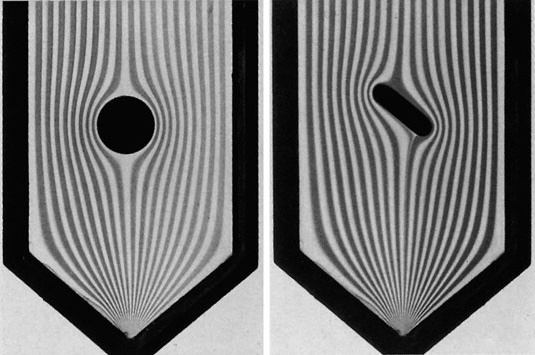
\includegraphics[height=6cm]{content/laminar.jpg}
		\caption{Laminare Strömungen.}
		\label{fig:laminar}
	\end{subfigure}
	\begin{subfigure}{4.46cm}
		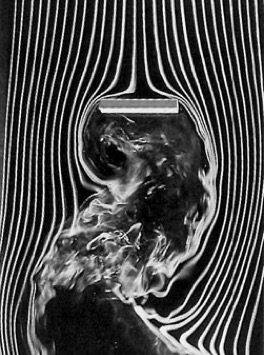
\includegraphics[height=6cm]{content/turbulent.jpg}
		\caption{Turbulente Strömung.}
		\label{fig:turbulent}
	\end{subfigure}
	\captionsetup{width=0.9\linewidth}
	\caption{Darstellung verschiedener Strömungsverläufe mittels Stromfädenapparat.
			 Einzelne Wasserschichten werden durch Einfärben sichtbar. Der Fluss
			 ist von oben nach unten gerichtet und wird über ein Ventil reguliert. \cite{dem_exp_1_8}}
	\label{fig:strömung}
\end{figure}

Der vorliegende Strömungstyp lässt sich über die dimensionslose Reynoldssche Zahl
\begin{equation}
	\symit{Re} = \pfrac{\rho v d}{\raisebox{0.7ex}{$\eta$}}
	\label{eqn:reyn}
\end{equation}
einordnen, wobei $v$ die relative Geschwindigkeit eines Körpers zur Flüssigkeit beschreibt und $d$ einer für das System
charakteristischen Länge entspricht. Wird dabei die kritische Reynoldszahl $\symit{Re}_\text{krit} \hspace{-0.15ex} \approx 2300$
überschritten, treten makroskopische Turbulenzen auf. Für Werte weit darunter überwiegt die laminare Strömung.

\newpage

\subsection[Kugelfallmethode im Höppler\hspace{0.15ex}-\hspace{-0.15ex}Viskosimeter]
		   {Kugelfallmethode im Höppler\hspace{0.15ex}-\hspace{-0.15ex}Viskosimeter \textnormal{\cite{viskos}}}

Im Wesentlichen besteht das Kugelfallviskosimeter aus einem transparenten, mit dem zu untersuchenden Fluid befüllten
Zylinder. In diesem befindet sich eine Kugel, deren Radius $r$ vernachlässigbar kleiner als der des Behälters ist.
Diese Differenz muss dennoch ausreichen, um die Bildung von Wirbeln zu verhindern. Damit weiterhin ein laminarer
Strömungsverlauf gewährleistet ist, wird der Zylinder leicht geneigt, sodass die Kugel an dessen Mantel herabgleiten
kann. Der entsprechende Winkel ist in der Fallbeschleunigung $g$ berücksichtigt. Als nach Gleichung~\eqref{eqn:reyn}
geforderte charakteristische Länge gilt in diesem System der Durchmesser $d = 2r$. Nun werden die wirkenden Kräfte
beim Fall der Kugel im Fluid betrachtet. Unter der Vorraussetzung laminaren Strömverhaltens ist die Reibung
\begin{align}
	F_{\hspace{-0.15ex}R} &= 6 \pi \eta v r
	\stepcounter{equation}\tag{2a}
	\label{eqn:stok} \\
	\intertext{gegeben, welche nach Stokes den Einfluss der einzelnen Flüssigkeitsschichten auf die Bewegung der Kugel
			   beschreibt. Zusätzlich setzt die Auftriebskraft}
	F_{\hspace{-0.3ex}A} &= \rho_\text{f\hspace{0.15ex}l} \hspace{-0.1ex}V\hspace{-0.05ex} g
	\tag{2b}
	\label{eqn:auf} \\
	\intertext{entgegen der Beschleunigung an, die von der Kugel als Resultat der Gravitation}
	F_{\hspace{-0.075ex}G} &= m g = \rho_\text{ob} \hspace{-0.1ex}V\hspace{-0.05ex} g
	\tag{2c}
	\label{eqn:grav}
\end{align}
erfahren wird. Dabei entspricht $v$ der Sedimentationsgeschwindigkeit, $V\hspace{-0.05ex} = 4/3 \, \pi r^3$ dient als
Bezeichner des Kugelvolumens. Mit den Dichten $\rho_{\text{f\hspace{0.15ex}l}}$ des Fluids und $\rho_\text{ob}$ des
sinkenden Objekts ergibt sich daraus die verdrängte sowie die verdrängende Masse. Nach kurzer Beschleunigungsphase
stellt sich die konstante Fallgeschwindigkeit $v_0$ ein. Dieser Vorgang begründet sich durch
das Eintreten eines Kräftegleichgewichtes, welches über
\begin{equation}
	F_{\hspace{-0.15ex}R} + F_{\hspace{-0.3ex}A} = F_{\hspace{-0.075ex}G}
	\label{eqn:glei}
\end{equation}
aufgestellt wird. Durch Umformen und Einsetzen lassen sich die äquivalenten Ausdrücke
\begin{align}
	F_{\hspace{-0.15ex}R} &= F_{\hspace{-0.075ex}G} - F_{\hspace{-0.3ex}A}
	\stepcounter{equation}\tag{4a} \\[2.1ex]
	6 \pi \eta v_0 r &=
	\rho_\text{ob} \hspace{-0.1ex}V\hspace{-0.05ex} g\hspace{0.05ex} -
	\rho_\text{f\hspace{0.15ex}l} \hspace{-0.1ex}V\hspace{-0.05ex} g
	\tag{4b} \\[0.8ex]
	\eta &= \pfrac{V\hspace{-0.05ex}g}{\raisebox{0.2ex}{$6 \pi v_0 r$}}
	\left( \rho_\text{ob} - \rho_\text{f\hspace{0.15ex}l} \right)
	\tag{4c}
\end{align}
schreiben, wobei Fallhöhe $x$ und Fallzeit $t$ über $v_0 = x \hspace{-0.15ex} / t$ verknüpft sind. Zusammenfassen
konstanter Größen erlaubt nun, den apparaturspezifischen Proportionalitätsfaktor
\begin{equation}
	K \propto K_0 = \pfrac{V\hspace{-0.05ex}g}{\raisebox{0.2ex}{$6 \pi r x$}}
	\label{eqn:kons}
\end{equation}
zu bestimmen. Die tatsächliche Gerätekonstante $K$ lässt sich auf diesem idealisierten~Weg allerdings nicht ermitteln,
da weitere Korrekturfaktoren einfließen. Ist $K$ dennoch bekannt, so kann durch Messen der Fallzeit die Viskosität
\begin{equation}
	\eta = K \left( \rho_\text{ob} - \rho_\text{f\hspace{0.15ex}l} \right) t
	\label{eqn:visk}
\end{equation}
berechnet werden.

\newpage

Eine temperaturabhängige Form der dynamischen Viskosität wird durch den Term
\begin{align}
	\eta &= A \exp \left( \pfrac{B}{\hspace{-0.15ex}T\hspace{0.15ex}} \right)
	\stepcounter{equation}\tag{7a} 
	\label{eqn:andr} \\
	\intertext{geliefert, die sogennante Andradesche Gleichung. Mit dem natürlichen \mbox{Logarithmus folgen}}
	\ln \left( \eta \right) &= \ln \left( A \right) + \pfrac{B}{\hspace{-0.15ex}T\hspace{0.15ex}}
	\tag{7b} 
	\label{eqn:andr_lin_1}\\[1.23ex]
	\ln \left( \pfrac{\eta}{\hspace{-0.05ex}A\hspace{0.05ex}} \right) &= \pfrac{B}{\hspace{-0.15ex}T\hspace{0.15ex}}
	\tag{7c}
	\label{eqn:andr_lin_2}
\end{align}
als zur inversen Temperatur linearisierte Varianten.

\subsection[Fehlerrechnung]{Fehlerrechnung \textnormal{\cite{unsicher}}}

Um die Abweichung der Messgrößen zu untersuchen, werden noch einige weitere Formeln benötigt.
Die Rechenvorschrift für den Mittelwert $\overline{x}$ ist mit
\begin{equation}
	\overline{x} = \pfrac{1}{N \,} \sum_{n=1}^N x_n
	\label{eqn:mittel}
\end{equation}
gegeben. Zur Bestimmung der Standardabweichung $\symup{\Delta}\overline{x}$ kann
\begin{equation}
	(\symup{\Delta}\overline{x})^2 = \pfrac{1}{N(N-1)} \sum_{n=1}^N (x_n \! - \overline{x})^2
	\label{eqn:std}
\end{equation}
verwendet werden. Durch die Gaußsche Fehlerfortpflanzung
\begin{equation}
	(\symup{\Delta}f)^2 = \sum_{n=1}^N
	\left( \! \pfrac{\partial^{\!} f}{\partial x_{\raisebox{0.2ex}{$\scriptstyle{n}$}}} \!
	\right)^{\!\! 2} \!\! (\symup{\Delta}x_{\raisebox{0.2ex}{$\scriptstyle{n}$}})^2
	\label{eqn:gauss}
\end{equation}
ist die Abweichung $\symup{\Delta}f$ für von fehlerbehafteten Werten $x_n \!$ abhängige
Größen $\hspace{-0.2ex} f \hspace{0.2ex}$ definiert.

\subsection[Lineare Regression]{Lineare Regression \textnormal{\cite{unsicher}}}

Entlang der linear abhängigen Messgrößen $(x_n,y_n)$ für $n = 1,\dotsc,\hspace{-0.1ex}N\hspace{0.1ex}$
lassen sich über
\begin{align}
	m = \pfrac{\overline{x\hspace{0.15ex}y\hspace{0.15ex}} - \overline{x} \: \overline{y\hspace{0.15ex}}}
	{\overline{x^2} - \overline{x}^{\hspace{0.15ex}2}} && b = \overline{y\hspace{0.15ex}} - m \overline{x}
	\label{eqn:regression}
\end{align}
die Parameter der Ausgleichsgerade $y = mx + b$ berechnen.
